%% ----------------------------------------------------------------
%% licenta.tex Fisierul principal
%% ----------------------------------------------------------------

\documentclass[a4paper, 11pt, oneside]{licenta}
\graphicspath{{Imagini/}}  % Folderul pentru imagini

% Pachete necesare
\usepackage[square, numbers, comma, sort&compress]{natbib}  % Folosim "Natbib" pentru bibliografie


\usepackage{fancyvrb}
\usepackage{color}



\makeatletter
\def\PY@reset{\let\PY@it=\relax \let\PY@bf=\relax%
    \let\PY@ul=\relax \let\PY@tc=\relax%
    \let\PY@bc=\relax \let\PY@ff=\relax}
\def\PY@tok#1{\csname PY@tok@#1\endcsname}
\def\PY@toks#1+{\ifx\relax#1\empty\else%
    \PY@tok{#1}\expandafter\PY@toks\fi}
\def\PY@do#1{\PY@bc{\PY@tc{\PY@ul{%
    \PY@it{\PY@bf{\PY@ff{#1}}}}}}}
\def\PY#1#2{\PY@reset\PY@toks#1+\relax+\PY@do{#2}}

\def\PY@tok@gd{\def\PY@tc##1{\textcolor[rgb]{0.63,0.00,0.00}{##1}}}
\def\PY@tok@gu{\let\PY@bf=\textbf\def\PY@tc##1{\textcolor[rgb]{0.50,0.00,0.50}{##1}}}
\def\PY@tok@gt{\def\PY@tc##1{\textcolor[rgb]{0.00,0.25,0.82}{##1}}}
\def\PY@tok@gs{\let\PY@bf=\textbf}
\def\PY@tok@gr{\def\PY@tc##1{\textcolor[rgb]{1.00,0.00,0.00}{##1}}}
\def\PY@tok@cm{\let\PY@it=\textit\def\PY@tc##1{\textcolor[rgb]{0.25,0.50,0.50}{##1}}}
\def\PY@tok@vg{\def\PY@tc##1{\textcolor[rgb]{0.10,0.09,0.49}{##1}}}
\def\PY@tok@m{\def\PY@tc##1{\textcolor[rgb]{0.40,0.40,0.40}{##1}}}
\def\PY@tok@mh{\def\PY@tc##1{\textcolor[rgb]{0.40,0.40,0.40}{##1}}}
\def\PY@tok@go{\def\PY@tc##1{\textcolor[rgb]{0.50,0.50,0.50}{##1}}}
\def\PY@tok@ge{\let\PY@it=\textit}
\def\PY@tok@vc{\def\PY@tc##1{\textcolor[rgb]{0.10,0.09,0.49}{##1}}}
\def\PY@tok@il{\def\PY@tc##1{\textcolor[rgb]{0.40,0.40,0.40}{##1}}}
\def\PY@tok@cs{\let\PY@it=\textit\def\PY@tc##1{\textcolor[rgb]{0.25,0.50,0.50}{##1}}}
\def\PY@tok@cp{\def\PY@tc##1{\textcolor[rgb]{0.74,0.48,0.00}{##1}}}
\def\PY@tok@gi{\def\PY@tc##1{\textcolor[rgb]{0.00,0.63,0.00}{##1}}}
\def\PY@tok@gh{\let\PY@bf=\textbf\def\PY@tc##1{\textcolor[rgb]{0.00,0.00,0.50}{##1}}}
\def\PY@tok@ni{\let\PY@bf=\textbf\def\PY@tc##1{\textcolor[rgb]{0.60,0.60,0.60}{##1}}}
\def\PY@tok@nl{\def\PY@tc##1{\textcolor[rgb]{0.63,0.63,0.00}{##1}}}
\def\PY@tok@nn{\let\PY@bf=\textbf\def\PY@tc##1{\textcolor[rgb]{0.00,0.00,1.00}{##1}}}
\def\PY@tok@no{\def\PY@tc##1{\textcolor[rgb]{0.53,0.00,0.00}{##1}}}
\def\PY@tok@na{\def\PY@tc##1{\textcolor[rgb]{0.49,0.56,0.16}{##1}}}
\def\PY@tok@nb{\def\PY@tc##1{\textcolor[rgb]{0.00,0.50,0.00}{##1}}}
\def\PY@tok@nc{\let\PY@bf=\textbf\def\PY@tc##1{\textcolor[rgb]{0.00,0.00,1.00}{##1}}}
\def\PY@tok@nd{\def\PY@tc##1{\textcolor[rgb]{0.67,0.13,1.00}{##1}}}
\def\PY@tok@ne{\let\PY@bf=\textbf\def\PY@tc##1{\textcolor[rgb]{0.82,0.25,0.23}{##1}}}
\def\PY@tok@nf{\def\PY@tc##1{\textcolor[rgb]{0.00,0.00,1.00}{##1}}}
\def\PY@tok@si{\let\PY@bf=\textbf\def\PY@tc##1{\textcolor[rgb]{0.73,0.40,0.53}{##1}}}
\def\PY@tok@s2{\def\PY@tc##1{\textcolor[rgb]{0.73,0.13,0.13}{##1}}}
\def\PY@tok@vi{\def\PY@tc##1{\textcolor[rgb]{0.10,0.09,0.49}{##1}}}
\def\PY@tok@nt{\let\PY@bf=\textbf\def\PY@tc##1{\textcolor[rgb]{0.00,0.50,0.00}{##1}}}
\def\PY@tok@nv{\def\PY@tc##1{\textcolor[rgb]{0.10,0.09,0.49}{##1}}}
\def\PY@tok@s1{\def\PY@tc##1{\textcolor[rgb]{0.73,0.13,0.13}{##1}}}
\def\PY@tok@sh{\def\PY@tc##1{\textcolor[rgb]{0.73,0.13,0.13}{##1}}}
\def\PY@tok@sc{\def\PY@tc##1{\textcolor[rgb]{0.73,0.13,0.13}{##1}}}
\def\PY@tok@sx{\def\PY@tc##1{\textcolor[rgb]{0.00,0.50,0.00}{##1}}}
\def\PY@tok@bp{\def\PY@tc##1{\textcolor[rgb]{0.00,0.50,0.00}{##1}}}
\def\PY@tok@c1{\let\PY@it=\textit\def\PY@tc##1{\textcolor[rgb]{0.25,0.50,0.50}{##1}}}
\def\PY@tok@kc{\let\PY@bf=\textbf\def\PY@tc##1{\textcolor[rgb]{0.00,0.50,0.00}{##1}}}
\def\PY@tok@c{\let\PY@it=\textit\def\PY@tc##1{\textcolor[rgb]{0.25,0.50,0.50}{##1}}}
\def\PY@tok@mf{\def\PY@tc##1{\textcolor[rgb]{0.40,0.40,0.40}{##1}}}
\def\PY@tok@err{\def\PY@bc##1{\fcolorbox[rgb]{1.00,0.00,0.00}{1,1,1}{##1}}}
\def\PY@tok@kd{\let\PY@bf=\textbf\def\PY@tc##1{\textcolor[rgb]{0.00,0.50,0.00}{##1}}}
\def\PY@tok@ss{\def\PY@tc##1{\textcolor[rgb]{0.10,0.09,0.49}{##1}}}
\def\PY@tok@sr{\def\PY@tc##1{\textcolor[rgb]{0.73,0.40,0.53}{##1}}}
\def\PY@tok@mo{\def\PY@tc##1{\textcolor[rgb]{0.40,0.40,0.40}{##1}}}
\def\PY@tok@kn{\let\PY@bf=\textbf\def\PY@tc##1{\textcolor[rgb]{0.00,0.50,0.00}{##1}}}
\def\PY@tok@mi{\def\PY@tc##1{\textcolor[rgb]{0.40,0.40,0.40}{##1}}}
\def\PY@tok@gp{\let\PY@bf=\textbf\def\PY@tc##1{\textcolor[rgb]{0.00,0.00,0.50}{##1}}}
\def\PY@tok@o{\def\PY@tc##1{\textcolor[rgb]{0.40,0.40,0.40}{##1}}}
\def\PY@tok@kr{\let\PY@bf=\textbf\def\PY@tc##1{\textcolor[rgb]{0.00,0.50,0.00}{##1}}}
\def\PY@tok@s{\def\PY@tc##1{\textcolor[rgb]{0.73,0.13,0.13}{##1}}}
\def\PY@tok@kp{\def\PY@tc##1{\textcolor[rgb]{0.00,0.50,0.00}{##1}}}
\def\PY@tok@w{\def\PY@tc##1{\textcolor[rgb]{0.73,0.73,0.73}{##1}}}
\def\PY@tok@kt{\def\PY@tc##1{\textcolor[rgb]{0.69,0.00,0.25}{##1}}}
\def\PY@tok@ow{\let\PY@bf=\textbf\def\PY@tc##1{\textcolor[rgb]{0.67,0.13,1.00}{##1}}}
\def\PY@tok@sb{\def\PY@tc##1{\textcolor[rgb]{0.73,0.13,0.13}{##1}}}
\def\PY@tok@k{\let\PY@bf=\textbf\def\PY@tc##1{\textcolor[rgb]{0.00,0.50,0.00}{##1}}}
\def\PY@tok@se{\let\PY@bf=\textbf\def\PY@tc##1{\textcolor[rgb]{0.73,0.40,0.13}{##1}}}
\def\PY@tok@sd{\let\PY@it=\textit\def\PY@tc##1{\textcolor[rgb]{0.73,0.13,0.13}{##1}}}

\def\PYZbs{\char`\\}
\def\PYZus{\char`\_}
\def\PYZob{\char`\{}
\def\PYZcb{\char`\}}
\def\PYZca{\char`\^}
\def\PYZsh{\char`\#}
\def\PYZpc{\char`\%}
\def\PYZdl{\char`\$}
\def\PYZti{\char`\~}
% for compatibility with earlier versions
\def\PYZat{@}
\def\PYZlb{[}
\def\PYZrb{]}
\makeatother




%% ----------------------------------------------------------------
\begin{document}

\frontmatter	  % Numerotare cu cifre romane( i, ii, iii, iv...)
% Titlul lucrarii
\title  {Operational monitoring of ATLAS TDAQ evolution}
\fstsupervisor  {\texorpdfstring
            {\href{rd.hersch@epfl.ch} {Prof. R.D. Hersch}}
            {Prof. R.D. Hersch}}
            
\sndsupervisor  {\texorpdfstring
            {\href{wainer.vandelli@cern.ch} {Wainer Vandelli}} 
            {Wainer Vandelli}}

\authors  {\texorpdfstring
            {\href{ctalau@cern.ch}{Cristian T\u al\u au}}
            {Cristian T\u al\u au }
          }
\UNIVERSITY  {\texorpdfstring{\href{http://epfl.ch}
                {\' Ecole Polytechnique Fédérale de Lausanne - EPFL}}
                {\' Ecole Polytechnique Fédérale de Lausanne - EPFL}}
\faculty     {\texorpdfstring{\href{http://ic.epfl.ch}
                {School of Computer and Communication Sciences}}
                {School of Computer and Communication Sciences}}
% \addresses  {\groupname\\\deptname\\\univname}
\date       {\today}
\degree     {Master Thesis}
\subject    {}
\keywords   {}

\maketitle


%% ----------------------------------------------------------------

\pagestyle{fancy}  % Folosim titlul sectiunii in antetul paginii
\tableofcontents

%% ----------------------------------------------------------------
\mainmatter	  % Numerotare normala (1,2,3...)

% Capitolele lucrarii
\chapter{Introduction} % Titlul capotilului
\label{Capitolul1}

\section*{System Overview}
The LHC (Large Hadron Collider) is a 27km circumference synchrotron that accelerates two counter rotating particle beams. The beams are collided at four interaction points for a contiguous period of 10-20 hours. The ATLAS detector (A Toroidal LHC ApparatuS) \citep{aad2008atlas}, designed for studying particles produced by proton-proton interactions and heavy ion collisions surrounds one of the interaction points. 

The image below presents a section of the detector which has a layered structure with the interaction point in the center of the detector. The different layers are specialized in measuring different properties of the particles as detailed in \citep{aad2008atlas}. 

\begin{figure}[ht!]
\centering
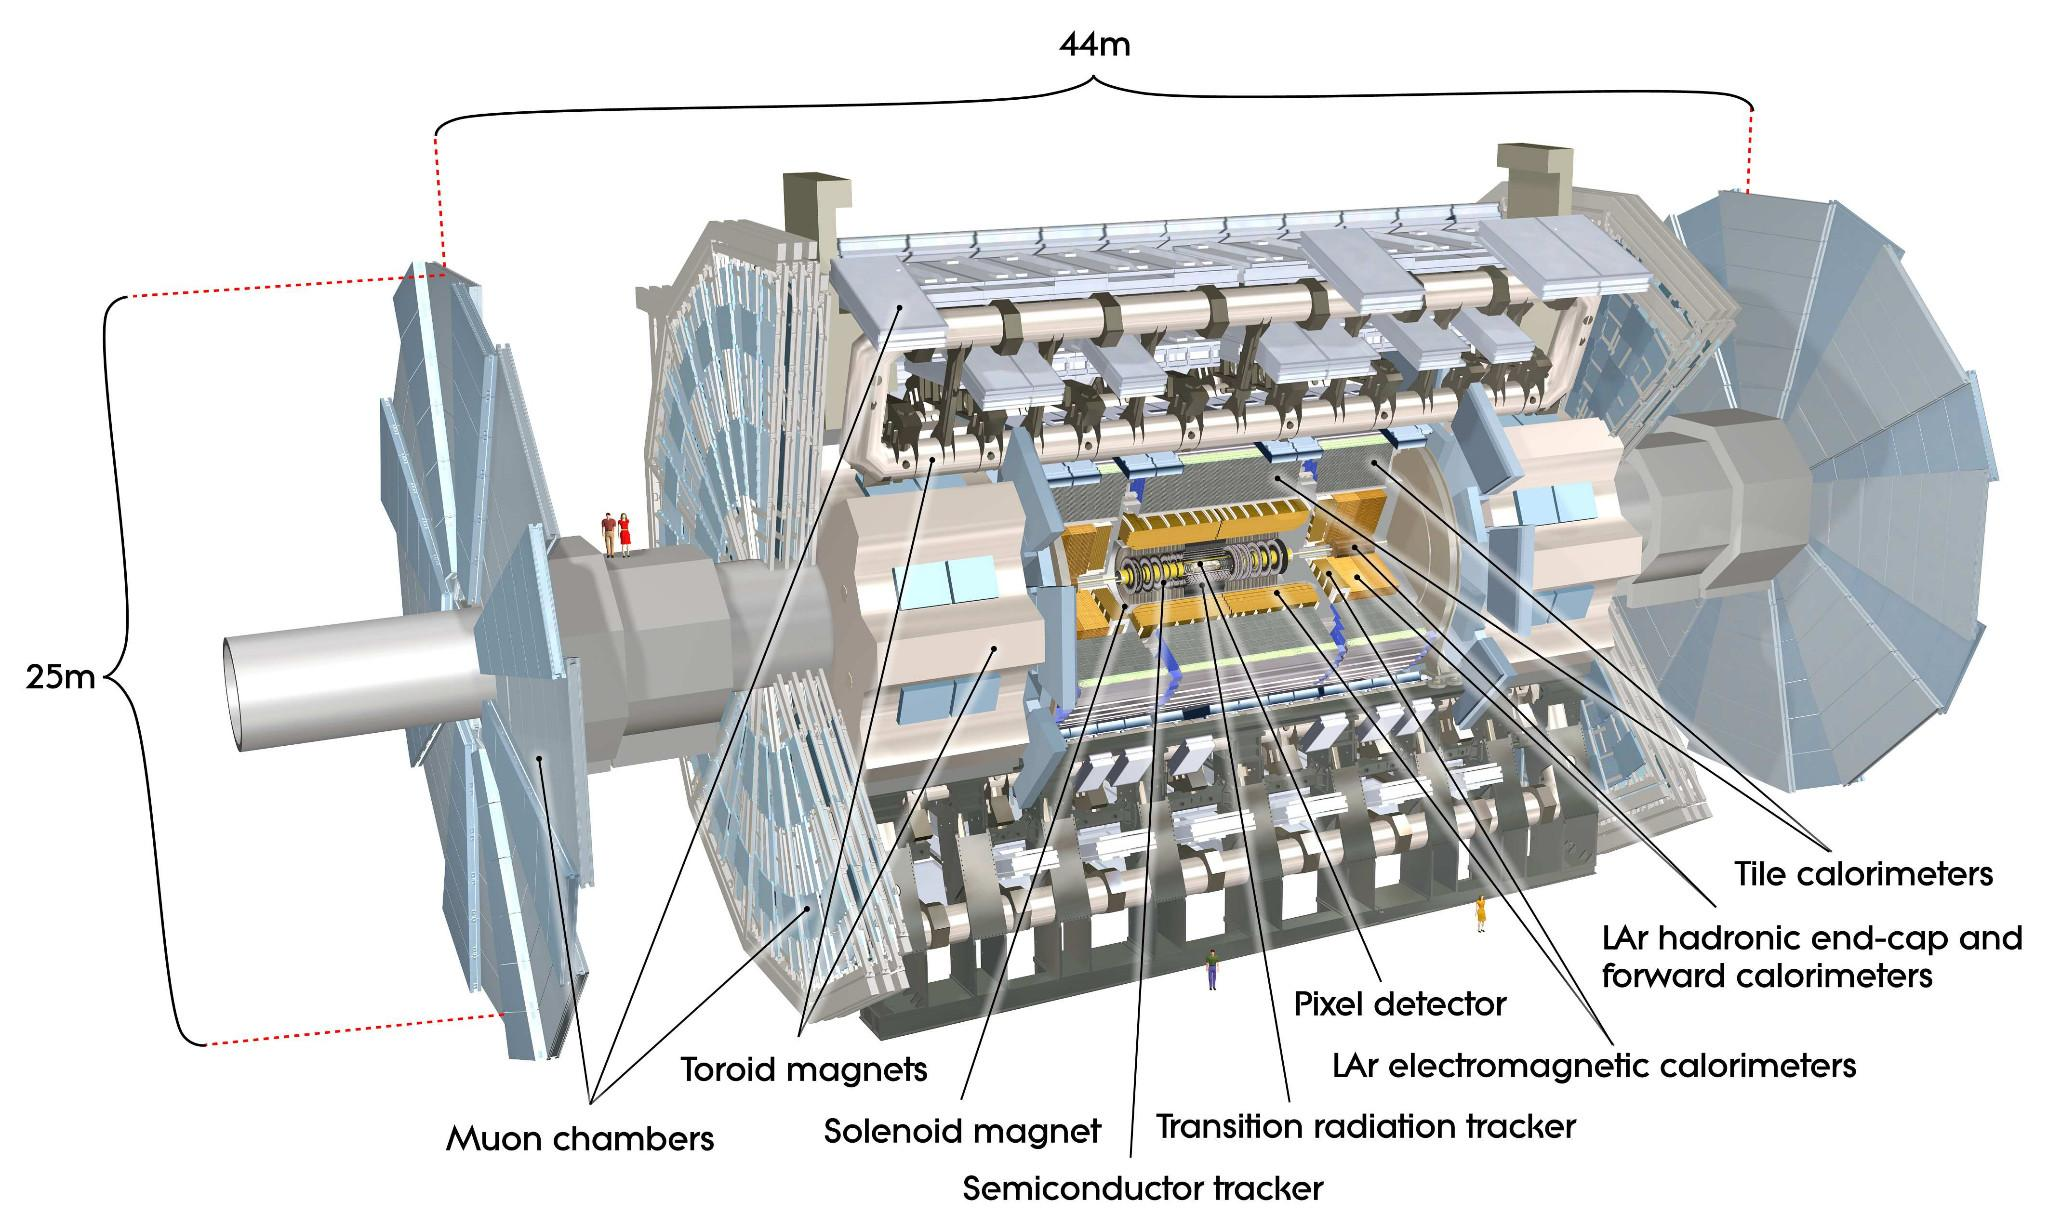
\includegraphics[scale=0.2]{Images/Overview.jpg}
\caption{ATLAS detector section view.}
\end{figure}


\section*{Event selection}
The two counter-rotating beams consist of trains of particle bunches. The distance between two consecutive particle bunches is around 25 ns and with the bunch crossing duration less than 1 ns. So bunch collision events happen with a frequency of 40MHz, each one consisting of 25 particle collisions in average. The data collected about these collisions has to be sent to the CERN persistent storage \citep{baud2003castor} for offline analysis. The amount of data collected for a single collision event is 1.5MB in average, which would mean a throughput of 60TB/s which is far more than what can be stored at a reasonable cost. Moreover, the number of events that are interesting for the offline analysis is only a small fraction of the total number of events. Hence, the events are filtered before being persisted using a three level data acquisition system (DAQ). 

\begin{figure}[ht!]
\centering
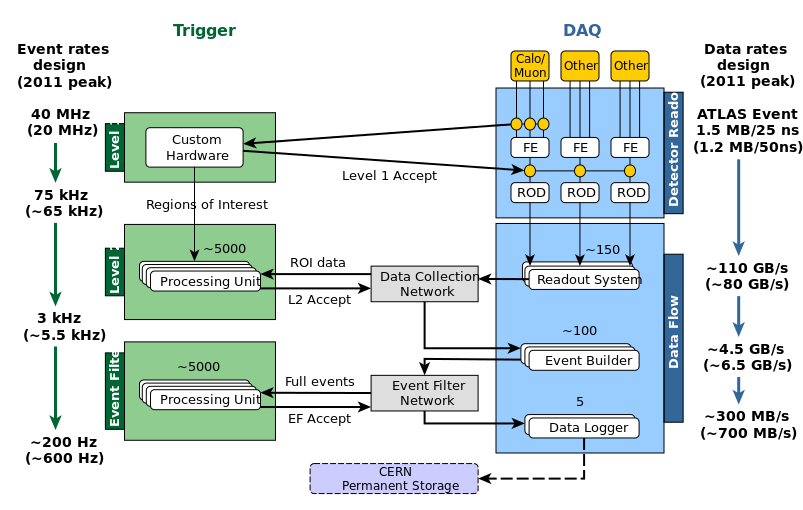
\includegraphics[scale=0.5]{Images/Trigger.png}
\caption{TDAQ system overview.}
\end{figure}

The first level trigger (L1) is built using custom hardware that can operate at 40 MHz and is placed as close to the actual detector as possible to reduce latencies caused by cable length. This level makes simple decisions based on the energy depositions in the calorimeters and of muon track segments in order to limit the latency to as low as 2.5 us. The acceptance rate of this level is chosen to be at most 75kHz. 

After being accepted by the L1, event data is stored in the ROBs (ReadOut Buffers) while it is processed by the second level trigger (L2) which is part of the HLT (High Level Trigger). The L2 reads only some parts of the data associated with an event (Regions of Interest or ROI) as hinted by the L1. The data used by the L2 system is in average 50KB per event and the latency of the order of tens of milliseconds. The L2 selection software is composed of more than 6000 instances of a software application running on 800 nodes, each of them handling one event at a time. 

Finally, the third level trigger, called Event Filter (EF) operates on the complete event data, at an input rate given by L2 of 3.5kHz. It has a configurable menu of more complicated selection algorithms and has a total latency of about 1 seconds and an acceptance rate of several hundred hertz which is within the mass storage limitations. The installation consists of 600 nodes running 6500 instances of the applications.

\subsection*{Evolution}

During the 2 year shutdown period starting at the beginning of 2013, a large upgrade of the entire system is planned \citep{hauser2012atlas}. In the DAQ system, the main change will be the merge of the L2 and EF.  

\begin{figure}[ht!]
\centering
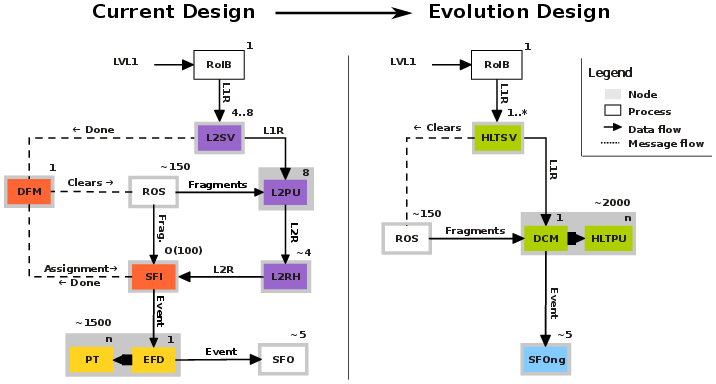
\includegraphics[scale=0.55]{Images/Evolution.png}
\caption{ATLAS TDAQ architecture evolution during shutdown.}
\end{figure}

All the applications dealing with event dispatching and other system management and control tasks (DFM, SFI, L2RH, EFD) will be merged into the HLT SuperVisor (HLTSV) and the DataFlow Control Manager (DCM). 
The L2 Processing Unit (L2PU) and the level 3 processing task (PT) will be merged into the HLTPU. In the new system instead of having L2 operating on chunks of event data and EF on whole events, we will have a series of algorithms that fetch event chunks incrementally as needed.

The main advantages of merging the two layers are better resource allocation, better load balancing and a simpler and more flexible system. However, assessing the benefits of this change needs validation in production mode with intensive operational monitoring.

\section*{Monitoring in ATLAS}

The ATLAS monitoring system \citep{collaboration2003atlas} is composed of information publishing libraries, information sharing services, monitoring facilities (e.g. that aggregate or persist monitoring information) and graphical displays.

There are two types of monitoring: operational monitoring which deals with operational data and functional parameters of different software and hardware components and event monitoring which monitors results of the analysis performed on events.

\subsection*{Components and services}

There are a number of components and services that play together in the monitoring system. We will present below the ones that have are the most relevant for operational monitoring starting from the lowest level ones up.

\begin{description}
\item[Inter-Process Communication (IPC) library \citep{corso2007data}] Is responsible for all the communication between applications in the ATLAS Trigger and Data AcQuisition (TDAQ)  system. It provides a much simpler interface to the underlying CORBA implementation including a simple API for the OMG Naming Service and a transparent cache for the remote object references.

\item[Object Kernel Support (OKS) database \citep{jones1998oks}\citep{alexandrov2001atlas}] Is an object-oriented database used for storing static configuration parameters for hardware and software components of the system, for example command line parameters and the node where to run a specific application. The data is loaded from XML data files and is validated against an user provided schema. 

In order to avoid overloading the database server during the system start and due to the static nature of the data, a system of caching proxies is used. This and the fact that the database does not have advanced query support enables it to meet the performance requirements of a real-time system.

\item[Partition editor] The software and hardware components in the TDAQ system are grouped in partitions which are configured using an OKS database. Due to the scale of the partitions (e.g. hundreds of applications), the configuration cannot be specified manually, but is automatically generated using a set of tools called partition editor.

\item[The ROOT framework \citep{brun1997root}] is an Object Oriented framework that contains among others an efficient file-based persistence mechanism, a C++ interpreter, reflection support, advanced statistical analysis instruments (multi dimensional histograms, fitting, minimization) and visualization tools. Most of the monitoring information in the system consists of such histograms.

\item[Information Sharing (IS) server \citep{kolosinformation}]  Is a server used to share monitoring information between applications that publish their own operational or event-related data and applications that need to process this information. The IS acts as an in memory key-value store, where keys are strings - the name of the objects - and values are subclasses of the ISInfo class. An application can read, write or update the information with a specific name. There is also the option for an application to subscribe to receive notifications when a value is updated. Due to the scale of our system, we run multiple instances of this server, each having its own name.

\begin{figure}[ht!]
\centering
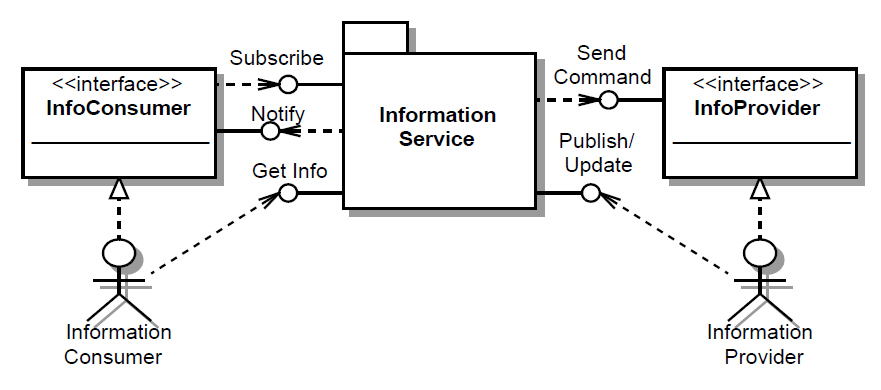
\includegraphics[scale=0.44]{Images/IS.png}
\caption{IS server interface.}
\end{figure}


The ISInfo class is intended to be a plain data structure with serialization and deserialization functions. They can be either written by the programmer or generated from an XML description.

\item[The Online Histogramming (OH) service \citep{kolosoh}] is a library which offers an interface to the IS server that allows one to store and retrieve ROOT histograms by transparently encoding them as ISInfo objects.

\item[The Gatherer \citep{renkel2010gatherer}] Is an application which aggregates monitoring information coming from different applications. For example, many applications track event data size distribution using histograms. The gatherer periodically reads all these histograms from the IS server, adds them and writes them back to the IS server. The aggregation is usually done in multiple stages, once per rack, and once globally across different IS servers. 

\item[Persistent Back-End for the AtlaS Tdaq (PBEAST) \citep{sicoe2012persistent}]: A Java application that persists operational monitoring data while storing the most recent data (1 month) in a queryable format. It subscribes to most of the IS servers and stores the updates in a Cassandra database.

\end{description}

\section*{Thesis structure}

The rest of the thesis report begins with a presentation of the project goal, namely the design and implementation of the {\tt monsvc} library. Then we describe the solutions for the challenges related to the \emph{configuration} of the library. In the next section, we present the algorithm used to \emph{schedule} the flow of monitoring information in the TDAQ network. Finally, we discuss some solutions for the \emph{synchronization} between the library which publishes the monitoring information and the application that updates it. The thesis ends with conclusions and possible future improvements.



\chapter{The {\tt monsvc} library} % Titlul capotilului
\label{Capitolul2}

The goal of my master project is to implement a library used by the applications to publish monitoring information to the IS servers \citep{kolosinformation}. This section is a brief overview of the functionality of the library. The following sections will present more details about specific aspects of the implementation such as configuration, scheduling and synchronization.

A data taking session of an LHC production fill lasts between 10 and 20 hours. During this time it is important to be able to monitor different operational parameters of the ATLAS TDAQ system and to react to abnormal conditions. For example, one needs to readjust parameters of the event selection software if the acceptance rate becomes so high that persistence services cannot handle it. 

To this end, all the applications in the system need to provide real-time updates about their operational conditions. These updates consist of (multidimensional) histograms, counters, rates, boolean variables, strings and collections thereof - we will refer to them as \emph{monitored objects}. Some examples of such objects are a counter of wrong checksums for event data read from the L1 filter or a histogram of the event sizes for the events accepted by the L2 filter. The updates are sent either periodically, or on demand: at the end of the run, when some exceptional condition occurs or when requested by the operator.

The {\tt monsvc} library takes care of the periodic publication of the monitored information, completely abstracting this task and leaving the application programmer in charge of solely updating the information with the current operational values. This is beneficial since the monitoring information is updated more often and more irregularly than it is published. For example, the counter of wrong checksums is updated every time such an error occurs, but it is expected to be published every 5 seconds. The interval between two publications of a monitored object is called call publishing interval.

In the monsvc approach, the monitoring is split into two operations: registration and publishing. The registration consists of passing a reference to an object to be monitored together with a name for that object to the monsvc library. The publishing deals with sending the data periodically to an IS server from where other applications will read it and either present it to the user or take corrective actions upon failures. 

The programmer needs to register the monitored objects (via the {\tt MonitoringService}), to configure the publishing process and to start it (via the {\tt PublishingController}). After this the programmer just needs to update the registered objects to reflect the current operational values. The image below presents an example workflow that the user may employ when working with the library.  

\begin{figure}[ht!]
\centering
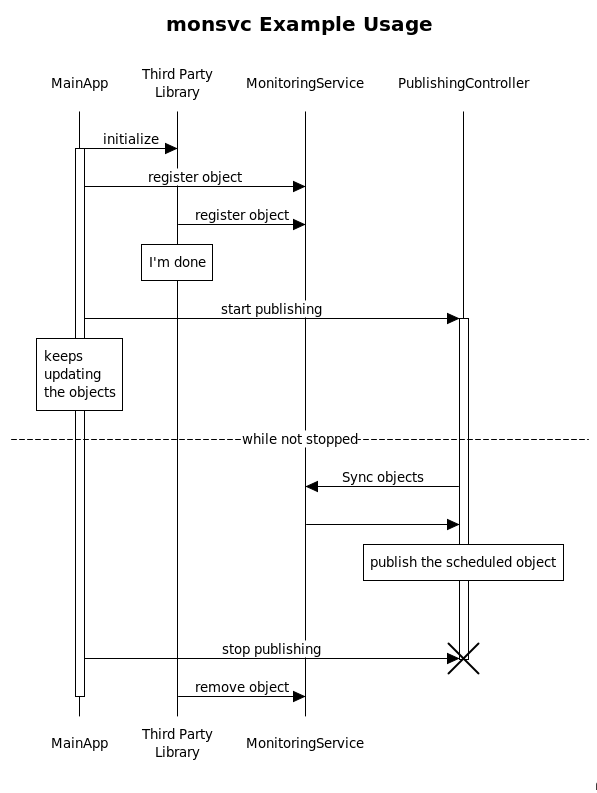
\includegraphics[scale=0.6]{Images/workflow.png}
\caption{{\tt monsvc} library usage example workflow.}
\end{figure}

The separation of registration and publishing also makes the life of third party library developers easier since their only job is to register the objects they want to be monitored while the main application is concerned with configuring and starting the publishing. For example, a network transport library will register information about the amount of trasferred data. This information will then be publsihed together with the main application data.

This usage pattern allows us to  create a lightweight version of the monsvc library with no transitive linking dependencies which contains only the registration functionality and which can be used by other libraries. The main application has to use the normal version which depends on a number of other packages like IPC, ROOT, IS, etc.


\chapter{Configuration} % Titlul capotilului
\label{Capitolul3}

\section{Introduction}

The applications in the ATLAS TDAQ system register up to several thousands of objects that represent information to be monitored. Different objects need to be published in different ways: for example with different publishing frequency and or to different Information Sharing (IS) servers or even need to be written to a file. As an example, the number of failed checksums of the event data read from the detector needs to be published every 10 seconds to an IS server called "L1". For another example, the histogram of accepted event data size should be written to a file called "DF.root" at the end of the running period. We aim to provide a way for the user to specify these parameters in an expressive, succinct and easy to use way. This process is called the \emph{configuration} of the library.

\section{Requirements}

The library allows the user to specify one or multiple \emph{publishing targets}. The publishing targets currently include IS servers, OH servers, files in ROOT format and standard output. For each target, the user can specify some \emph{publishing parameters}, for example, the name of the IS server and the publishing interval for an IS publishing target.

Another important functionality is to be able to modify the configuration at runtime. For example, if an operator notices some abnormal conditions in the running of the system, she may enable some debug monitoring information to be published in order to identify and fix the problem. 

\section{Challenges}

As with other parts of the system, the main challenge of the configuration is the scale of the system. We discuss below how each dimension of scaling impacts the design of the library.

\subsection*{The code size}

First of all, in order to publish a monitored object, the library needs to know the publishing parameters. The first decision to be made is whether to associate the parameters with the objects programmatically (in the source code), or in an external file which is loaded at runtime. We chose the second approach since, any change in the source code requires a recompilation and to create a binary patch of the current release version of the software. The duration and complexity of this process would discourage developers from changing configurations. In the external file approach, a change in configuration can be as simple as editing a text file and checking it in in the source repository.

\subsection*{The number of monitored objects}

With over 5000 monitored objects, we need to keep the configuration file of an application within a manageable size. We leverage the fact that the objects fall into a few semantic categories that share publishing requirements. We define groups of objects that share the same publishing parameters by using regular expressions. 

\begin{figure}[ht]
\centering
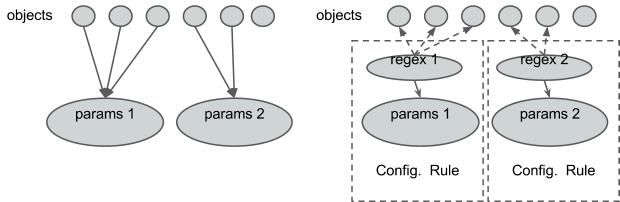
\includegraphics[scale=0.6]{Images/oks_regex.png}
\caption[Publishing parameters association.]{The two approaches for associating publishing parameters with monitored objects: explicit (left) and implicit by using regular expressions (right).}
\label{fig:oks_regex}
\end{figure}

As presented in the figure \ref{fig:oks_regex}, instead of having explicit links from the monitored objects to sets of parameters, we create links from parameters to objects by using configuration rules. A configuration rule is composed of a regular expression and a set of parameters. It is this rules that we store in the configuration file. A nice side-effect of this approach is that if the programmer registers a new object which uses an existing parameter set, she just has to give it a name that matches the regular expression.

One problem related to the object sets specification as regular expressions is that it is not easy to express exceptions from a rule. For example: we want to publish histograms with names matching {\tt “DEBUG/.*”} every 10 seconds, but we have a really big histogram among them that we would like to publish less often. To this end, we chose to add an exclude filter to every configuration rule that specifies the exceptions to that rule.

\subsection*{The number of developers}

In order to avoid complicated link time dependencies between packages, we adopted the split responsibility model: the developer of a library (other than {\tt monsvc}) registers some objects and the developer of the application (which uses the library) is the one who needs to configure their publishing parameters. Since some objects are registered by one developer and configured by another one, a clear convention should be used between the two. 

Our configuration mechanism allows the library developer to provide configuration rules for the objects registered by its library. To this end we created the concept of rule bundle which contains configuration rules and links other rule bundles. With this approach the developer of the main application can just link the rule bundle of the library from the rule bundle of the application. This mechanism handles nicely transitive dependencies by using transitively linked bundles.

The configuration files are a set of interlinked XML files, one per application or library. These files form the configuration database which can be loaded at run time by using the OKS system. The database is an object oriented one, where for example every application is described by a {\tt PublishingApplication} object which has a one to one relation to a rule bundle which is represented by an object of class {\tt ConfigurationRuleBundle}. The complete schema of the configuration database is presented in figure \ref{fig:oks_schema}. 

\begin{figure}[ht]
\centering
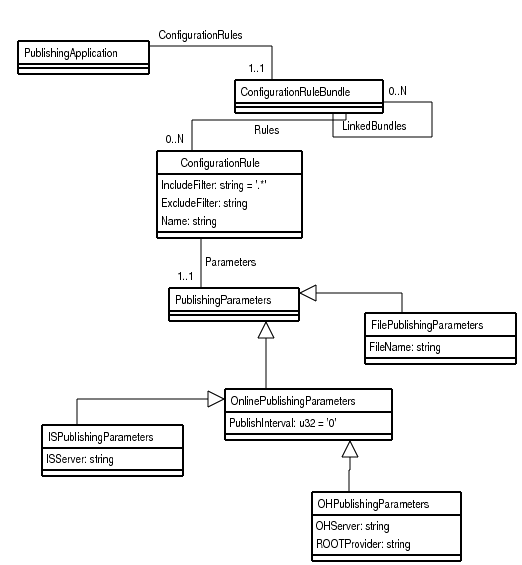
\includegraphics[scale=0.75]{Images/oks_schema.png}
\caption{Configuration database schema.}
\label{fig:oks_schema}
\end{figure}

\subsection*{The number of application instances}

Some applications in our system have several thousands of instances which use similar configuration files with only a few configuration parameters that differ. For example, if every application writes the objects in a file, then the name of the file should be different for the applications running on the same node. These configuration files are generated automatically from a common template using the partition editor tool.

Another challenge is related to the configuration changes during a running period. Our solution uses IS commands mechanism to allow the human operator to send the configuration change commands to the IS server which forwards them to the applications.

\chapter{Scheduling} % Titlul capotilului
\label{Capitolul4}


In this section we discuss the scheduling problem which consists of choosing the publishing time for every object registered with our library on every application instance. We first identify the objectives of the scheduling algorithm, present some solutions and assess them by using both a simulation and a test-bed deployment of the system. 

\section*{System overview}

Our monitoring system is composed of 12000 applications which send data to 32 multithreaded IS servers.  All these applications are instances of 15 binaries, most of them being L2 and EF selection applications. Instances of the same application have the same set of registered objects.

Since applications talking to different IS servers are independent, we chose to model a system with a single IS server and 400 applications that run on 40 nodes. The communication is done using CORBA \citep{vinoski1997corba}, the server has 8 threads by default and runs on a machine with 12 CPUs. We also assume that every application sends most of its data to a single IS server in the same rack connected in the same switch with a 1Gbps connection.

A typical example of monitored objects set is the one of the Event Filter nodes which monitor 5138 histograms with an average of 438 bins per histogram. For L2 nodes, there are 5087 histograms with 1126 bins in average. The publishing interval is usually configured between 1 second and 10 minutes. Although applications publish also many kinds of objects such as counters or flags, most of the published monitoring information consists of histogram. Since histograms have the biggest influence the performance of the system I will use the name histogram to refer to any kind of such object.

\section*{Publishing requirements}

\begin{description}
\item[Minimize jitter.]

First of all, we should be able to publish each histogram periodically, with the interval between two consecutive publications approximately equal to the interval configured by the user. We should be able to handle multiple publishing intervals. A number of intervals of the order of 10 is expected.

Let's consider a histogram with publishing interval $I$ and let the time of the $k$-th publication of a histogram be $T_k$; we call $J=\max(\lvert T_k-((k-1) \cdot I+T_1\rvert)$ the jitter of the histogram. We want to have $J < 0.1\cdot I$ for every histogram.

\item[Minimize latency.]

We publish the histograms using a separate thread from that of the main application which does the event filtering. In this thread we call a black-box function that takes care of all the details of sending the histogram to the IS server (buffering, marshaling, etc.). We have to keep the histogram locked while we are calling this function in order to prevent a concurrent access from the thread that is updating the histogram. As the application may block waiting for the histogram to be published instead of doing useful work, we want to minimize the publishing latency.

\item [Minimize publishing skew.]

Collision event data is distributed to all the applications, each maintaining its own histograms about the processed events. These histograms are evolving in time and in order to have an overview about the system’s operational state we need to take a snapshot of the histogram from all nodes at some point in time and to aggregate them.

In order to take a snapshot of a histogram across all nodes at some point in time, we need to have all nodes publishing their instance of that histogram with minimal skew. The publishing skew of a histogram is defined to be the difference between the moments when the first and the last instance of the histogram is received by the IS server.  

\item [Maximize throughput]

We want the published information in the IS server to be as fresh as possible. So we need to publish as many histograms per second as possible allowing the user user to configure smal publishing intervals.

\item [Efficient incremental reconfiguration]

We want to allow the users to reconfigure the system at runtime, which means that our schedule should incorporate the new changes on the fly. We want to implement this feature as efficient as possible which means we don’t want the system to stop publishing for a long time in order to apply the new configuration changes. 

We also want that if we change the publishing interval for some histograms, the rest of them should continue to be published according to the same schedule as before.

\item [Avoid bursty traffic]

A bursty traffic pattern seen by the IS server impacts the overall system performance in multiple ways. First, it requires big inbound queues both in IS server and in all the upstream applications to which the IS server pushes information. 

Another effect is related to the IS subscriber applications that use garbage collection for memory management. They are known to suffer from periodic freezes \citep{aho2007compilers}, but more recent garbage collection algorithms \citep{printezis2005garbage} are designed to work in parallel with the application as long as it doesn’t allocate memory at a very high rate which is exactly what bursty traffic causes.

Although important, this requirement has the same cause as the first one, namely contention, so we will treat it as a secondary one.

\end{description}

\section*{Global and local scheduling}

The previously identified requirements can be split into two classes. The first class consists of the requirements that can be satisfied by each application intance in isolation, we call them local requirements. These are the jitter minimization and reconfiguration efficiency. 

As it can be seen from the requirements above, although the instances of applications that use the monsvc library do not communicate explicitly, they affect each other’s performance by creating contention in the monitoring network of the ATLAS TDAQ system. Indeed, requirements like skew and latency minimization and bursty traffic avoidance are global requirements that can be satisfied only if the application instances cooperate.

If we consider the time as being divided in equal length slots, we can think of local scheduling as assigning which histograms are published in which slot and the global scheduling as when to publish the histograms within a time slot. 

The slot size choice is not simple since it has many conflicting requirements, but on the positive side it does not depend on the configuration, so it has to be changed only when there are big changes in infrastructure (hardware and network) or when the distribution of histograms sizes changes fundamentally.

This separation also helps us in presenting to the users a simple model for configuring the publishing intervals. The system reports the number of available slots per second and the users need just to calculate how many slots per second their rules require. The users, however, should not expect 100\% utilization of the slots due to irregularities of the publishing intervals set.

\section*{Global scheduling}

For this problem we assume that we every application has the same set of histograms to publish in a particular time slot. The set of histograms is very small, ideally only one histogram, but due to the imperfection of the local scheduling there can be several of them.

We have to satisfy two conflicting requirements, namely publishing skew and latency minimization. In order to minimize publishing skew we should try to make all the applications publish simultaneously. But this practice will create contention in the IS server and the latency will increase. 
The strategy that we adopted for this problem is to make each application choose the moment of the publishing randomly within the first part of the time slot of length $f\cdot I$, where $f<1$ is a configuration parameter and $I$is the size of the time slot.

In order to deal with the case in which the interval is too short for publishing all the histograms, we extend it until we are done publishing everything and reduce the length of the next interval.

An example of scheduling is depicted below, where we have three applications that start the publishing within the first $f=0.75$ part of the interval.

\begin{center}
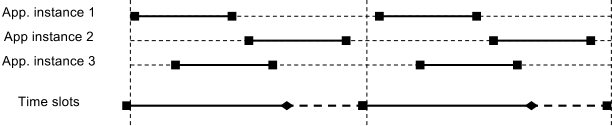
\includegraphics[scale=0.6]{Images/local_sched.png}
\end{center}

Since we have no communication between applications our solution has a very low overhead and is fault tolerant. It is also robust with respect to the clock skew as long as it is small enough (smaller than 1ms). Another advantage is that by tuning the $f$ parameter we can trade-off between skew and latency. 

\section*{Real-time formulation of local scheduling}

The local requirements for our scheduling requirements can be viewed as a real-time scheduling problem \citep{liu1973scheduling}, \citep{sha2004real}. In order to make this more apparent, we establish the following mapping of concepts:
\begin{itemize}
\item Each of the $n$ histograms is considered a task that generates jobs periodically. 
\item A job means to publish the histogram to the IS server.
\item The latency of a publishing a histogram corresponds to the execution time of a job $C_i$.
\item The publishing interval is the task period $T_i$. 
\item The maximum jitter of a histogram is the deadline of the corresponding job $D_i=0.1\cdot T_i$.
\item The IS server has a similar role to the CPU that need to be scheduled among the tasks.
\item The throughput of our system is the utilization of the corresponding real-time system.
\end{itemize}

\subsection*{Related work}

In the real-time scheduling literature there are two main classes of algorithms: static ones in which the priority of a task is determined before the system is started and dynamic ones in which the priority of a task can change dynamically. 

The most popular static algorithm is the Rate Monotonic Scheduling (RMS) \citep{liu1973scheduling} in which the priority of a task is higher for tasks with small periods. The algorithm is preemptive, so when a task with small period becomes available, the ones with larger period are preempted and it starts running. Another variation is Deadline Monotonic Scheduling which gives higher priority to tasks with shorter deadlines. In our case, we cannot preempt a histogram from being published, so this algorithms are not applicable. 

Among the dynamic algorithms, we mention Earliest Deadline First (EDF) \citep{liu1973scheduling} in which, whenever the processor is idle and some tasks are available, we start the task whose deadline comes first and run it up to completion. This algorithm is optimal in the sense that if a system is schedulable with some algorithm, then it is also schedulable with EDF.

People concentrated on developing criteria to check whether a real-time system is schedulable with these algorithms. For EDF the condition XXX is that the utilization $U < 1$ and the following holds:

$$ \forall L > 0.\,  \sum_{i=1}^n \left\lfloor \frac{L+T_i-D_i}{T_i}\right\rfloor C_i \le L $$

which in our case, for $C_i=10$ms, $T_i=5$mn, $L=D_i=30$s, $n=5000$, becomes:

$$ \sum_{i=1}^n 1 \cdot C_i \le L \Leftrightarrow 50s \le 30s $$

Note that the utilization in our case is $U=\sum_{i=1}^n\frac{C_i}{T_i}=n\frac C T = \frac 1 6 = 0.166$ which is very low. 

For DMS in order to check the schedulability, we have to determine the worst case response time for every task using the following recursive equations XXX.

 $$ \forall i.\, R_i=C_i+\sum_{j=1}^{i-1} \left\lceil \frac{R_i}{T_i} \right\rceil \cdot C_j \Leftrightarrow R_i = i\cdot C$$
 
 So, again, the response time for the last histogram is $R_n=n\cdot C=50s >D_n=30s$. We can notice that since all the histograms have the same period they have the same priority so they are published sequentially. So, in order to satisfy the deadlines with this algorithm we should be able to publish all the histograms in 10\% of the time. Note that having higher priorities for some of the histograms does not improve the situation of the ones with low priority.

\subsection*{Offset-free systems} 
 The common assumption of these algorithms that render them ineffective for our system is that all histograms should start to be published in time slot 0. However, this is not necessary in our case, so, we have more degrees of freedom in choosing the time offset at which the first publication of each histogram occurs. Multiple choice strategies are presented in the literature about offset-free systems \citep{goossens2003scheduling}, \citep{grenier2008pushing}.
 
In \citep{goossens2003scheduling} the author proves a number of useful results about offset-free systems and presents two algorithms for assigning offsets to a set of tasks. The first algorithm finds an optimal offset assignment and it has a complexity of $O(n^2 \cdot \frac{\prod_{i=1}^n Ti}{\text{lcm}(T_i)})$ which renders it useless for any practical purpose. The second algorithm is an heuristic one which runs in $O(n^2\cdot \log(\max_{i=1\ldots n}(T_i)))$ and has space complexity $O(n^2)$. The algorithm works by considering pairs of tasks in decreasing order of greatest common divisor of their periods and trying to assign offsets such that the jobs of these two tasks are as distant as possible. The limitation of this algorithm is that it looks only at one other task offset before making the choice of the offset.

In the context of scheduling messages in CAN networks, Grenier et al. \citep{grenier2008pushing} propose another heuristic algorithm which runs in $O(n\cdot \max_{i=1 \ldots n}(T_i))$ and has better experimental results than the previous one. The algorithm tries to assign offsets such that the first job of every task is as far as possible from other jobs. It does this by considering tasks in the increasing order of their periods and assigns the offset such that the first job of task is as far as possible from every job of a task that was assigned so far. The drawback of this approach is that the algorithm does not look at the subsequent jobs of a task and it creates collisions (two jobs scheduled for the same time) even for simple scenarios.

Once the offsets have been chosen, we still have to design a scheduling algorithm. For offset-free systems, the DMS algorithm is no longer optimal among static algorithms but an optimal priority assignment can be found with $O(n^2)$ time complexity \citep{audsley2001priority}. On the other hand, among dynamic algorithms EDF is still optimal. 

\section*{Hash based offset assignment}

A simple offset assignment algorithm chooses the offsets by hashing the names of the histograms and taking the value modulo their period. In order to have histograms with different names published with small skew one can configure an identical \emph{hashing name} which, if present, is used instead of the histogram name to determine the time slot 

This strategy ensures that every application will assign the same offset to a histogram even if they have different histogram sets. However, this situation can only occur when we change the configuration at runtime and only for brief periods. Another positive aspect is that the reconfiguration can be done in $O(1)$ time: we just assign offsets to the changed histograms and keep the existing ones unchanged.

The problem of this algorithm is that even for a perfect hashing function the expected maximum number of histograms assigned to a single slot is $O(\frac{\log n}{\log \log n})$ \citep{mitzenmacher1996power}. They will overload the IS server, will overflow to the next time slots and increase the publishing skew. On the other hand, the expected number of empty slots is newhich gives us a throughput of 63\% of the maximum.

\section*{Subperiod offset assignment algorithm}

In this section we present a heuristic algorithm that leverages the particularities of our system to assign offsets for histogram with no jitter, no collisions and high throughput. 

In our configuration files, all the periods are expressed in seconds which means that the greatest common divisors among periods are large - equal to the number of slots per second which is 30-50. Moreover, large subsets of histograms have periods which are multiple of 5 or 10 seconds. We will also take advantage of the fact that we have only a few (5-10) distinct periods in order to achieve better time complexities for offset assignment.

\subsection*{Terminology}

It is proved in \citep{goossens2003scheduling} that we can choose the offset for a histogram to be less than its period without loss of generality. 

In the context of a single histogram, its offset determines a set of slots. For example, an offset $k$ for a histogram with period (i.e. publishing interval) $P$ means the slots $\{k+n\cdot P | n \geq 0\}$. Note that in the definition, the period was implicitly defined by the histogram. If the period cannot be derived from the context, we explicitly mention it: offset $k$ modulo $P$.

\subsection*{Intuition and pseudocode}

The algorithm operates in two steps. First it repeatedly approximates unions of histogram groups with different periods with one group having a smaller period until we are left with only one group. Then we start with this group and assign offsets recursively to groups that it approximates until we get to assign offsets to all histograms.

At the beginning every histogram will form its own group:
\begin{verbatim}
group = {period : histo.period, n : 1, offset : None}
\end{verbatim}
In order to describe the approximation operation let’s assume that our configuration include two histogram groups: one having 4 histograms to be published every 10 sec. and another one 4 histograms to be published every 15 sec. So, we need to assign 4 offsets in the range [0s, 10s) and 4 offsets in the range [0s, 15s).
 
Let’s consider the time being divided in 5 sec subperiods. Denote by x the number of offsets from the first group that are chosen in the interval [0s, 5s) and by y the number of those in the interval [5s, 10s). Similarly, denote by a, b, c the number of offsets from the second group in the three 5 seconds subperiods of the interval [0s, 15s). In the figure below we represented the number of slots used to publish histograms in 6 consecutive subperiods of 5 sec:

\begin{center}
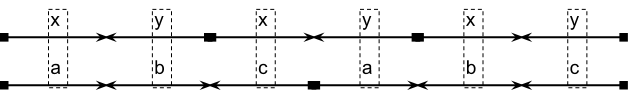
\includegraphics[scale=0.6]{Images/subperiod.png}
\end{center}

We have a fixed number of slots per second, so we have a bound on the number of slots that we can use in each of the subperiods. In order to stay within this bound our strategy is to minimize the maximum number of used slots in a subperiod. In our case this reduces to the following optimization problem:
$$ \text{minimize } \max(x+a, y+b, x+c, y+a, x+b, y+c) \text{ subject to } a+b+c=4 \text{ and } x+y = 4 $$
One can easily prove that:
$$ \max(x+a, y+b, x+c, y+a, x+b, y+c) = \max(x, y, z) = \max(a, b, c)$$
So, we only need to minimize the maximum number of slots used in a subperiod for each of the two task groups. The minimum of 4 slots is achieved if we distribute the offsets uniformly among subperiods of 5 sec, that is, choosing $x=2, y=2$ and $a=2, b=c=1$. With this setting we can (over-)approximate the union of the two groups with one (synthetic) group of 4 histograms to be published every 5 sec.

In general the following function computes the approximation of two groups:
\input{Code/approximate}
The \verb+sons+ store the groups that it approximates together with their maximum number of slots per subperiod.

This is an over-approximation in the sense that if we can assign offsets for the resulting group, then we can also assign offsets for the initial groups. Let’s assume we have assigned offsets $\{o_1,o_2,o_3,o_4\}$ to the four histograms in the synthetic group. We can allocate offsets $\{o_1, o_2\}$ modulo 5 sec for the first group and offsets $\{o_3, o_4\}$ modulo 5 sec. Note that these offsets are the same with $\{o_1, o_2, o_1 + 5, o_2 + 5\}$ modulo 10 sec and $\{o_3, o_4, o_3 + 5, o_4 + 5, o_3 + 10, o_4 + 10\}$ modulo 15 sec. These two offset sets can now be recursively assigned to the 4 histograms in each of the groups. The general algorithm is presented in pseudocode below:
\input{Code/assign}
The next function converts the offset list from offsets modulo subperiod to offsets modulo \verb+period+:
\input{Code/expand}
A sketch of a possible algorithm execution is presented in the figure below, where we have 5 histograms with period 2 sec, 4 histograms with period 10 sec. and another 4 histograms with period 15 sec. The blue rectangles represent the initial histograms and the purple ones represent approximating groups. The strategy of choosing the next pair of groups to approximate determines the shape of the tree.
\begin{center}
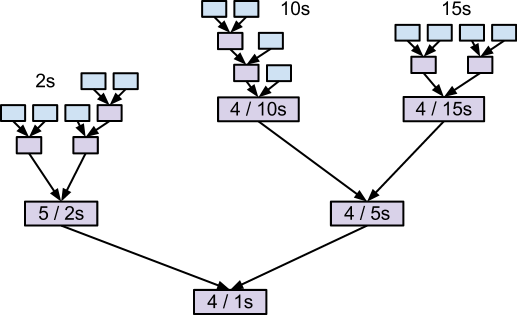
\includegraphics[scale=0.6]{Images/subperiod_tree.png}
\end{center}
Now we just need to assign offsets to the root group and they will be pushed up to the histograms in the leafs:
\begin{verbatim}
assign(build_tree(groups), offsets)
\end{verbatim}

\subsection*{Incremental version}

In the algorithm presented above we assign a set of offsets to the root group of the tree and it takes care of pushing subsets of it to its child nodes, which recursively push subsets of them up the tree until they reach the leafs where they are assigned to histograms. We leave unused offsets along the way. For example, in order to assign 4 offsets to the group with period 15 sec we need to allocate 2 slots modulo 5 sec. from the parent node that actually which actually mean 6 offsets modulo 15 sec leaving us with 2 unused offset modulo 15 sec.

When a new histogram is added, it is attached to the tree as a leaf. Next, we should locate some unused offsets in the tree and try to push them towards the node corresponding to that histogram. However, it is simpler to use a pull model in which the node corresponding to the newly added histogram is pulling an unused offset from its parent. If the parent has no unused offsets, it tries to pull one from its parent and so on, until the root is reached. At this point algorithm fails if there are no unused offsets.

We associate an OffsetSupply to each of the groups to hold its unused offsets. Initially all the supplies are empty except from the root whose buffer is pre-filled with all the offsets modulo its period. When a node pulls an offset from its parent supply, it converts it to multiple offsets modulo its period.
\input{Code/offsetsupply}
The algorithm for adding a histogram is the following:
\input{Code/addhisto}
If this incremental addition of a histogram to the tree with pull-based offset assignment succeeds, the previously assigned offsets are preserved. However, this incremental changes to may determine a sub-optimal tree structure. So, if the algorithm fails, as a last resort, we rebuild the tree from scratch and possibly change all previously assigned offsets.

\subsection*{Complexity analysis}

In this section we will discuss the tradeoff between the complexity of the strategy to choose the next pair of groups to approximate and the quality of the resulting schedule.

Let’s first introduce a quality measure for a subperiods tree built by our algorithm. 

\begin{definition}
Definition. For a node with period $P$ whose parent node has period $P_1$ we define the maximum number of offsets modulo 1 sec. wasted along the edge between the two nodes to be $c(P_1,P)=\frac{1}{P_1}-\frac 1 P$.
\end{definition}

This maximum is achieved if the child pulled a slot from its parent, so it reserves $\frac P {P_1}$ slots modulo $P$, and delivered only one slot to its children. This means $\frac P {P_1}-1$ wasted slots every $P$ seconds, which is $\frac 1 {P_1}- \frac 1 P$ wasted slots per second. 

\begin{definition}
The total maximum number of unused slots for a tree is $c(T)=\sum_{e\in T}c(e)$. 
\end{definition}

For convenience we call these numbers the cost of an edge and of a tree respectively. A strategy is better than another one if it produces trees with smaller cost. 

Note that this measure is very conservative. First because we assume that the worst case happens for every edge which usually is not the case. Second, because that these slots are wasted by our algorithm when compared to a perfect schedule that uses $\frac 1 P $ slots for a histogram with period $P$. Even an optimal schedule that satisfies the deadlines of our system wastes some slots compared to this perfect schedule. Finally, these slots are not entirely wasted - they can be used when we add new histograms incrementally.

\subsubsection*{NP-completeness of optimal strategy}

Equipped with these definitions, the problem of building an optimal tree for $n$ histogram groups with periods $P_1, P_2, \ldots,P_n$ can be formulated as follows. Let’s consider the graph with vertices denoted by numbers $1,2,,P=\max_{i=1,\ldots,n}(P_i)$ with edge between the vertices $a, b$ of cost $\frac 1 b -\frac 1 a$ if $b \vert a$; find the minimum-cost tree that contains vertices $P_1,\ldots,P_n$ and $\gcd(P_i)$.

We can notice that this problem is an instance of the Directed Steiner Tree optimization problem which is NP-hard and the with standard complexity assumptions there exists no approximation algorithm with a ratio better than $\frac {\ln (n)} 4$ \citep{zelikovsky1997series, ming2006fasterdsp}.

We will prove that our problem is also NP-hard by reducing from the Bounded Frequency Set Cover problem \citep{gary1979computers, cmulecture}. In fact, since our problem has numeric inputs we will prove it strongly NP-hard \citep{garey1978strong}, that is, it is NP-complete even if the numeric inputs, i.e. the periods, are bounded by a polynomial in the input size.

The Bounded Frequency Set Cover (BFSC) problem for $B \ge 2$ is the following: Given a finite set $X=\{x_1,\ldots,x_q\}$ and a collection of its subsets $C=\{C_1,\ldots, C_n\}$ such that each $x_i$ occurs in at most $B$ subsets, does it contain a subcollection of size kthat covers the set $X$?

Now, let’s present the polynomial time reduction from the Bounded Frequency Set Cover to our problem. Let’s associate with every $C_i$ a prime number $p_i$ and with every $x_i$ a set of histograms with period $Pi=\prod_{x_i\in C_k}p_k$.

We can choose $p_i$ to be the $2\cdot r+i$-th prime number, so according to [25] it will satisfy $2\cdot r <p_i<2\cdot 3r \ln 3r$ where $r=\max(n, q)$ and we will be able to bound the periods by a polynomial in the input size, for example $P_i=O(r^{B+1})$. In order to establish the reduction we just have to prove the following theorem. 

\begin{theorem}
The optimal tree for this set of histograms with periods $P_i$ has the cost between $k-0.5$ and $k+0.5$ if and only if to the BFSC instance has a subcover of size $k$ for $k \ge  1$.
\end{theorem}

First we prove an useful lemma which says that the cost of the tree is concentrated in the edges connected to the root node which has period 1.

\begin{lemma}
The cost of a subtree that contains $k$ leafs and whose root is $p$ has the cost at most $\frac{k}{p}$.
\end{lemma}

\begin{proof}
We proceed by induction on the number of nodes. If there is only one node, it is a leaf and the cost of the tree is $0<\frac 1p$. Otherwise, the root has two children with periods $p_1$ and $p_2$ that have $k_1$ and $k_2$ leafs in the corresponding subtree. The cost of the tree is: 

\begin{eqnarray*}
c(p) &=& \left(\frac 1p - \frac 1 {p_1}\right) + \left(\frac 1 p - \frac 1 {p_2}\right)+c(p_1)+c(p_2) \\
    &\leq & \frac 2p-\frac 1 {p_1}-\frac 1 {p_2} + \frac {k_1}{p_1}+\frac {k_2}{p_2} \\
    &=&\frac 2p + \frac{k_1-1}{p_1}+\frac{k_2-1}{p_2} \\
    &\leq & \frac{k_1+k_2}p \\
    &=&\frac kp
\end{eqnarray*}

We applied the induction hypothesis for the subtrees starting at $p_1$ and $p_2$ which are smaller. 
\end{proof}

\begin{proof}[Proof of Theorem]
We will prove the two parts of the equivalence between the two problems separately:
\begin{description}
\item[Opt. strategy $\Rightarrow$ BFSC] 
Since our tree has the cost between $k-0.5$ and $k+0.5$ it means that it has at exactly $k$ edges incident to the node 1 because their cost is $k-\sum{j=1}^k \frac 1 {p_j} \geq k-\frac k {2r} \geq k-0.5$ and the cost of the rest of the tree is $ <\frac k {p_1}< \frac r{2r}<0.5$ according to the lemma we just proved. Let $D_1, \ldots, D_k$ be the neighbors of the root. For each of them, the leafs in its subtree are divisible with $D_i$, so they are divisible with one of its prime divisors $p_{i_j}$, so they are contained in $C_{i_j}$. Hence, the subcollection $C_{i_j},j=1,\ldots,k$ is a subcover of size k.

\item[BFSC $\Rightarrow$ Opt. strategy] Let’s consider a subcover $\{C_1,\ldots,C_k\}$. The tree in which the root is connected to the nodes $p_i$ which are connected to leafs $P_j$ for which $p_i \vert P_j$ has the cost $c$ which satisfies the relations: $c > \sum_{i=1}^k 1-\frac 1{p_i} > k-\frac k{2r}>k-0.5$ and according to the lemma $c<\sum_{i=1}^k 1-\frac 1{p_i}+0.5<k+0.5$.
\end{description}\end{proof}
 
Following the same lines we can prove that even a strategy that chooses a minimal number of neighbors for the root is NP-hard to find.

\subsubsection*{Heuristic strategy}

In this section I will present a heuristic strategy to compute a near optimal subperiods tree with reasonable complexity. 

A first step is to approximate not only pairs of groups but also multiple groups with the same period. It is easy to see that all k histograms with period Pcan be approximated (exactly) by a group of khistograms and period P. Before building the tree we can create these groups in $O(n)$ leaving us with only mnodes to be processed by the \verb+build_tree+ function. 

In the \verb+build_tree+ function we can then consider the pairs of groups in decreasing order of their common subperiod. In order to implement this function efficiently we use a priority queue:

\begin{verbatim}
def build_tree(groups):
  subperiods = priority_queue(lambda (g1, g2): gcd(g1.period, g2.period))
  for g1, g2 in cross_product(groups, groups):
    subperiods.add((g1, g2))
  while len(groups) > 1:
    g1, g2 = subperiods.popmax()
    groups -= [g1, g2]
    g’ = approximate(g1, g2)
    for g in groups:
      subperiods.remove((g1, g))
      subperiods.remove((g2, g))
      subperiods.add((g’, g))
    groups += [g’]
  return groups[0]
\end{verbatim}

Since we have mgroups of histograms at the beginning, we end up with $2m-1$ groups in the entire tree. So, the number of pairs inserted in the priority queue is at most $O(m^2)$ since we don’t insert the same pair twice. The number of removals is at most as big, and the number of times the maximum is popped is $O(m)$ since we have at most miterations in the while loop. The of each of these operations is $O(\log m^2+T)$, the second term coming from the  computation. So, the total complexity of the \verb+build_tree+ function is $O(m^2(\log m + \log T))$. 

\subsubsection*{Offset assignment complexity}
For the complexity analysis of the offset assignment I will use the pull version presented in the previous section. I assume that the offset buffer of the \verb+OffsetSupply+ is built lazily, so its construction and pop operation are $O(1)$. I also assume that in $O(m)$ we merge all nodes with their parents that have the same period.

Let’s estimate the cost of making $k$ pull operations from the offset supply $s$. Let’s denote its ancestors by $s_i,i=1,\ldots,l$ and let the period of $s_i=d_1\cdot\ldots\cdot d_i$ where $d_1=1, d_i \geq 2$. It is easy to see that the pull operations from the offset supply $s_i$ will have to call the pull method of $s_{i-1}$ every ditimes. We can easily the following recurrence for the cost of $k$ pull operations on the node $s_i$.

$$ f(s_i, k) = k + f\left(s_{i-1}, \left\lceil \frac k {d_i} \right\rceil \right)$$

The solution of this recurrence is:

\begin{eqnarray*}
f(s_l,k) &=& k+ \left\lceil \frac k {d_l} \right\rceil + \left\lceil \frac k {d_l\cdot d_{l-1}} \right\rceil + \ldots + \left\lceil \frac k {d_l\cdot \ldots d_2}\right\rceil \\
         &<&l+k+\frac k {d_l}+ \frac k {d_l\cdot d_{l-1}} + \ldots \\
         &\leq & l+k+\frac k 2+\frac k 4 + \ldots \\
         &<& m+2k
\end{eqnarray*}

So, the complexity of all $n$ pull operations from moffset supplies associated $w$ ith mdistinct nodes is $O(m^2+n)$ and the complexity of an incremental change which adds $k$ histograms with the same period is $O(m+k)$. 

\subsection*{Scheduling algorithm}
The scheduler should return for every time slot the histogram that was assigned to that time slot. In order to speed up the scheduling decisions we split histograms into groups according to their period and sort them by offset inside each group. 

\subsubsection*{Heap-based scheduler}
One possible implementation of the scheduler is to use a min-heap to hold the next histogram to be published from each group, ordered by the time of publishing. After a histogram is popped from the heap, the next one for that group is added. This approach has a complexity $O(\log m)$ per scheduling decision which is low enough for our purpose. The space complexity is $O(m)$.

\subsubsection*{Table-based scheduler}

We can implement the scheduler with only $O(1)$ time complexity per scheduling decision at the price of higher space complexity. The common approach is to precompute the schedule for a time duration equal to the least common multiple of the periods. Since we do not have collisions, we can improve over this approach by storing only a small window of the future schedule as a circular buffer. The schedule decision consists of removing and returning the histogram at the beginning of the buffer and adding the next histogram from the same group at its corresponding position.
 
The buffer size is equal to the greatest interval between two offsets of histograms having the same period. This is $O\left(\frac {m \cdot T}  n\right)$ in expected value and $O(T)$ in the worst case, where $T=\max_{i=1,\ldots,n}(T_i)$.

\subsubsection*{Incremental schedule changes}

In order not to stop the publishing for too long while making changes to the histogram configuration, we can continue publishing according to the old schedule until the new offsets are all assigned in another thread using the previously described algorithm. Only when we know all the offsets, we stop the scheduler and commit the changes.

This technique allows us to have smooth incremental changes even when the subperiod tree is rebuilt - process that runs in time $O(n+m^2(\log m+\log T))$. The actual complexity of changing the table-based scheduler is $O(m)$ for a complete offset reassignment and $O(1)$ for incremental changes. For the heap-based one, the times are $O(m\log m)$ and $O(m)$ respectively.

\section*{Experimental results}
How real experiments differ from simulation.
How do they scale with the number of nodes.
How to tune parameters.
How it is better than the previous system.

\subsection*{Simulation}

\subsection*{Testbed measurements}
\subsubsection*{Jitter measurements}
\subsubsection*{Traffic shaping}
\subsubsection*{Publishing skew and latency}




\chapter{Synchronization} % Titlul capotilului
\label{Capitolul5}

\section{Introduction}

As described in chapter \ref{Capitolul2}, the applications that use our library are take care of updating the monitored objects with the current operational values while in a separate thread the {\tt monsvc} library samples these objects and sends them to an IS server. Since some of the monitored objects are not thread-safe, for example ROOT histograms, this concurrent access pattern creates problems which include issues regarding visibility of updates of one thread in another one and accessing data structures in inconsistent state. Therefore, we need to synchronize the access to the monitored objects between application and library threads.

\section{Smart pointers}

We use smart pointers in order to implement the synchronization between the application and the library while requiring only minimal and incremental changes to the existing codebase. For every object registered with the library we return a smart pointer that is used by both library and application as a proxy for accessing the registered object. 

The smart pointers offer a simple interface to the application developer. They have two functions called lock and unlock which ensure exclusive access to the underlying object. Moreover, we use an interesting C++ feature \citep{andrei2001modern} that allows us to overload the dereference operator to lock the smart pointer just before any method call or field access and unlock it afterwards.

Due to the nice syntactical similarities between smart pointers and raw pointers we can easily port the code to use the former. It usually requires just changing the type of the declaration of the pointer. For example, the following function can be ported just by changing the type of the parameter:
\input{Code/dow1}
to obtain the following form:
\input{Code/dow2}
As explained above, the smart pointer takes care of the synchronization with the library on every function call and field access.

There is an exception to the previous case in which the pointer should be passed to a legacy function which we cannot change. For example:
\input{Code/dow3}
in which case we replace it with:
\input{Code/dow4}
Note that in this case even the change was very small, there is a trade-off between lock granularity and the amount of code that needs to be changed. For example, if we had ten calls to legacy functions and each of them was fast, we could as well lock around the \verb+do_work+ to save the refactoring work.

\section{Synchronization policies}

In the previous section we referred to locking and unlocking the smart pointer without giving details about how this is implemented. In this section we will present different implementations among which the application developer can choose when registering an object.

\subsection{No synchronization}

The information that is stored in the IS server is represented as objects with the base class ISInfo. Some of these objects are generated from XML description. We implemented a script which can generate a thread-safe version of the object which uses atomic integers for the fields. 

In cases where this level of thread-safety is sufficient, a developer can avoid the overhead of locking by using a smart-pointer that provides no synchronization.

\subsection{Mutex}

The simplest synchronization policy is to acquire mutex when accessing the object. The disadvantage of this policy is that the library has to lock the object while it sent over the network to the IS server. This is because the publishing to the IS server uses a legacy function similar with the example we have given before.

\subsection{Copy before publish}

When using this synchronization policy, the library makes local copy of the object before publishing it to the IS server. The advantage of this technique is that we avoid holding a lock while sending the object over the network. The disadvantage is that we consume more time and memory to make a copy of the object which may not be acceptable for large histograms.

This policy is the opposite of copy-on-write but we prefer it since in our case the object is written more often than is read.

\subsection{Asynchronous updates}

An important observation which we can leverage is that in our use cases, the application that updates an object with the current operational values does not need to wait for the update to be applied. All we are interested in is serial consistency of the operations on that object. 

With the asynchronous updates policy, we still use a mutex to ensure exclusive access to the underlying object. The only difference is that when the application tries to update a locked object it just enqueues the update to be applied at a later time. Our updates usually increment a counter or a histogram bin, hence they can be represented very compactly making this strategy lightweight in terms of space usage. It also avoid blocking the main application threads while sending the monitored objects over the network.

The interface of the smart pointer that implements this strategy leverages the C++11 variable argument templates to provides asynchronous updates to any type of monitored object. The declaration of the method responsible with asynchronous updates is the following:
\input{Code/async_ptr}

This method takes a pointer to a member function and its arguments and calls it asynchronously. It requires to change the method calls of the from \verb+h->observe(42)+ to use the following form: \verb+h.async(Histo::observe, 42);+.

Another positive point of this implementation is that we can rewrite only some of the method calls to be asynchronous, so there is again a trade-off between the amount of code to be modified and performance.

\subsubsection*{Intuition}

The figure \ref{fig:sync_ptr} represents the operation of the locking strategy while the figure \ref{fig:async_ptr} corresponds to the asynchronous updates strategy. One can see that in the second case, the application thread is not disturbed by the monitoring thread which is publishing the object that it is trying to update.
\begin{figure}[ht!]
\centering
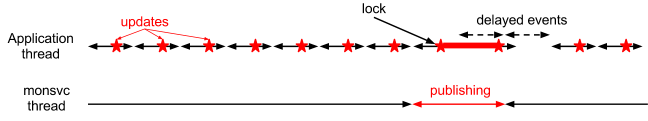
\includegraphics[scale=0.6]{Images/async_before.png}
\caption{Locking strategy}
\label{fig:sync_ptr}
\end{figure}

\begin{figure}[ht!]
\centering
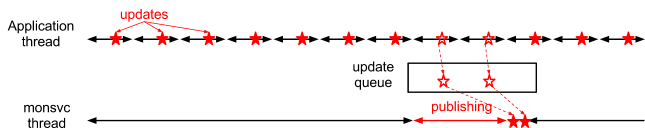
\includegraphics[scale=0.6]{Images/async_after.png}
\caption{Asynchronous updates strategy}
\label{fig:async_ptr}
\end{figure}

\subsubsection*{Implementation}

In this section we will present the implementation of the main operations of the smart pointer. The dereference operator is implemented on top of these operations. The smart pointer class has the following fields:
\begin{itemize}
\item {\tt update\_queue} the queue of updates that need to be executed asynchronously.
\item {\tt qlock} a mutex used to protect the {\tt update\_queue}.
\item {\tt obj\_lock} a mutex used to protect the object pointed by the smart pointer.
\end{itemize}
And the pseudocode is given below:
\input{Code/async}
Note that the {\tt async} method does not block when trying to acquire {\tt obj\_lock} since it uses the non-blocking {\tt try\_lock} method. 

Every thread that acquires the {\tt obj\_lock} mutex executes all updates that were added to the {\tt update\_queue} before accessing the underlying object of the smart pointer. This way we ensure that after the exclusive access to the object is given to the application, the object is in a serially consistent state. As an optimization, we also execute all updates before releasing the {\tt obj\_lock}.

\subsection{Custom mechanisms}

We also provide a smart pointer that uses callbacks to allow user to implement its own synchronization mechanisms such as, for example, per-cpu counters that are added up only before being read.

%% ----------------------------------------------------------------
\backmatter

\setstretch{0.9}  % Spatierea intre linii de 0.9 - o singura pagina de bibliografie
\addtocontents{toc}{\vspace{2em}}  % Spatiu in cuprins inainte de bibliografie

\label{Bibliografie}
\lhead{\emph{Bibliography}}  % Headerul paginii este "Bibliografie"
\bibliographystyle{unsrtnat}  % Stilul "unsrtnat"
\bibliography{bibliografie}  % Fisierul cu bibliografia

% Todo-uri in faza de lucru
%\todos
\end{document}
%% ---------------------------------------------------------------- 